\section{Cross-domain error complementarity}
\label{sec:cross-domain}
Historical cross-domain scores can conceal two different properties: whether the systems make \emph{complementary} errors, and whether their \emph{agreement} is trustworthy. We examine all 28 main suites without pooling across their 15 source collections or reference standards. For a suite $s$, let $c_{im}$ denote reference agreement of system $m$ on typed decision $i$. We define the best observed single-system rate $b_s=\max_m\operatorname{mean}_i c_{im}$ and the reference-aware oracle ceiling $u_s=\operatorname{mean}_i\max_m c_{im}$. Their difference $u_s-b_s$ is \emph{selection headroom}, not the gain of a trained or deployable router: the oracle uses each decision's reference to choose a system. Separately, a strict five-system majority exists only when at least three valid outputs are the same label. We report its coverage and conditional error risk, retaining failures in the fixed five-system panel. Pointwise intervals resample source/state clusters within each suite.

Figure~\ref{fig:cross-domain} reveals why the two properties should not be conflated. On SST-5 with the choice interface (dataset-provided reference), the best observed system reaches 55.9\% agreement and the oracle ceiling 87.3\%, a 31.4-point gap (95\% cluster interval [28.5, 34.4]); nevertheless, strict majority covers only 78.6\% of decisions and errs on 42.7\% of those covered (interval [39.3, 46.1]). On Aegis2 prompt annotations (human-reference track), oracle headroom is 16.0 points [14.4, 17.7], while majority covers all decisions but has 26.0\% error [24.1, 28.0]---8.4 points less reference agreement than the best observed system (paired interval [$-10.5$, $-6.4$]). The opposite geometry also occurs: on the programmatic Jev--Laya needle suite, oracle headroom is only 0.3 points [0.0, 0.7] while majority risk is 21.3\% [13.0, 30.1] at 99.8\% coverage; that suite has 900 decisions but only 25 original content clusters. A high oracle ceiling thus identifies \emph{potential} error complementarity, not a consensus-based way to realize it. Because system selection, examples and analytical questions were developed after the historical outputs existed, these are exploratory within-suite descriptions, not evidence that a cross-domain selector would generalize.

\begin{figure}[p]
\centering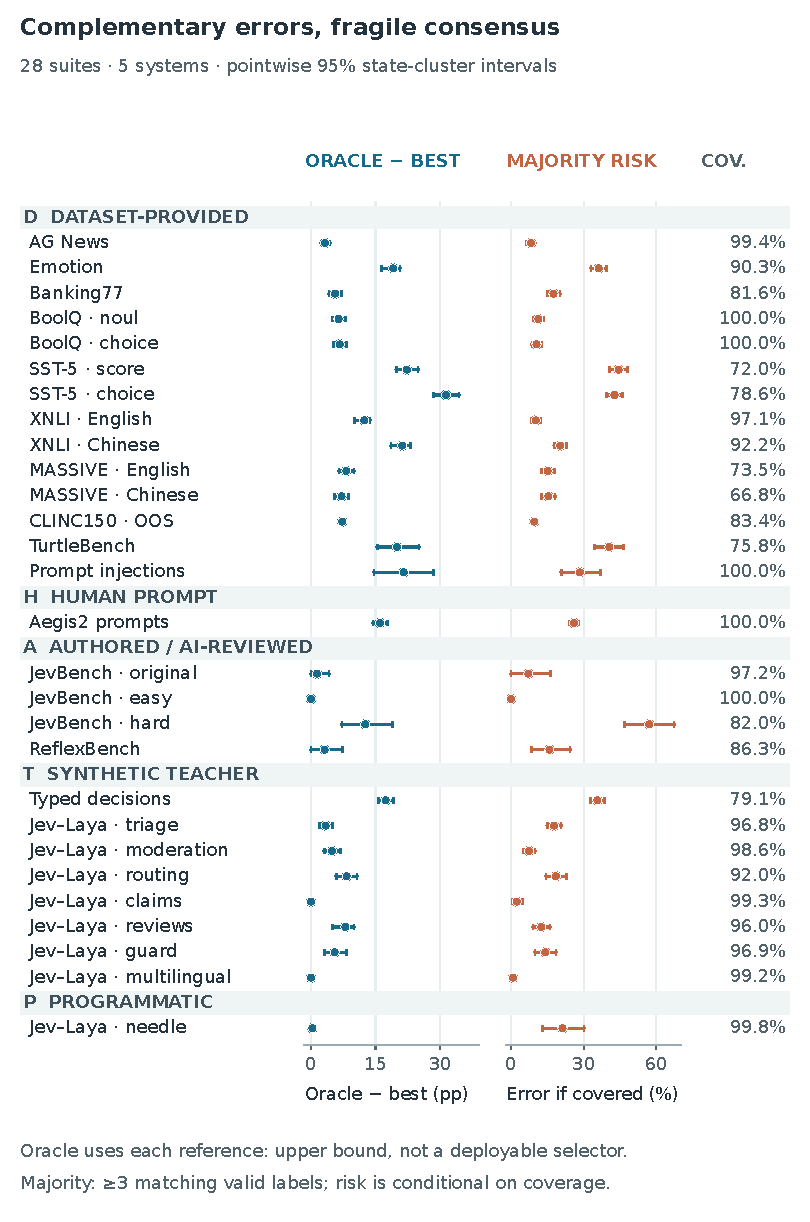
\includegraphics[width=.99\linewidth,height=.84\textheight,keepaspectratio]{figures/fig_cross_domain_main.pdf}
\caption{Selection headroom and strict-majority risk across 28 main suites, grouped by reference provenance: D, dataset-provided; H, human prompt; A, authored or AI-reviewed; T, synthetic teacher; P, programmatic. Left: the reference-aware oracle ceiling minus the best observed system, \emph{not} an attainable router gain. Right: error conditional on at least three identical valid labels, with coverage in the adjacent column. Whiskers are pointwise 95\% state-cluster bootstrap intervals (5,000 draws). Shared-source variants are not independent; no across-source inference is made.}
\label{fig:cross-domain}
\end{figure}
